\documentclass{beamer}
\usetheme{metropolis}
\usepackage{graphicx}
\usepackage{subfig}
\usepackage{tcolorbox}
\title{Algebra-Based Physics-2: Electricity, Magnetism, and Modern Physics (PHYS135B-01): Review}
\author{Jordan Hanson}
\institute{Whittier College Department of Physics and Astronomy}

\begin{document}
\maketitle

\section{Review}

\begin{frame}{Summary}
\begin{enumerate}
\item Chapter 18 - Charges and Electric Fields
\item Chapter 19 - Electric Potential and Electric Field
\item Chapter 20 - Electric Current, Resistance, and Ohm's Law
\item Chapter 21 - Circuits and DC instruments
\item Chapter 22 - Magnetism
\item Chapter 23 - Electromagnetic Induction
\item Electromagnetic waves
\end{enumerate}
\end{frame}

\begin{frame}{Review}
\begin{columns}[T]
\begin{column}{0.5\textwidth}
\small
Charge $q_1 = 2$ nC and $q_2 = 1$ nC.  Find the location on the x-axis with an E-field value of 0, if $q_1$ and $q_2$ are each 20 cm from the origin. \\ \vspace{0.5cm}
Suppose $q_1 = 1$ nC and $q_2 = 1$ nC.  What is the right expression for the E-field a distance $r$ that is far away from the origin?
\begin{itemize}
\item A: $E = k (q)/r^3$
\item B: $E = kq^2/r^2$
\item C: $E = k q/r^2$
\item D: $E = 2k q/r^2$
\end{itemize}
\end{column}
\begin{column}{0.5\textwidth}
\begin{figure}
\centering
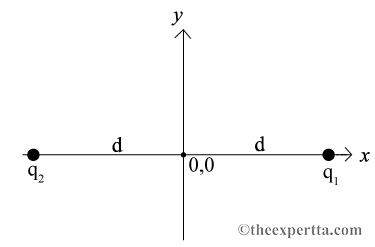
\includegraphics[width=0.95\textwidth]{ex1.png}
\caption{\label{fig:ex1}}
\end{figure}
\end{column}
\end{columns}
\end{frame}

\begin{frame}{Review}
\begin{columns}[T]
\begin{column}{0.4\textwidth}
\small
Suppose the density of the oil droplets in the Millikan oil-drop experiment is 885 kg/m$^3$.  If the radii of the drops is observed to be 1 $\mu$m, what is the mass of the drops? \\ \vspace{0.5cm}
What is the weight of the drops in Newtons? \\
\vspace{0.5cm}
Suppose an E-field of 4545 N/C is required to hold the drops motionless.  How many electrons are on the drops, on average?
\end{column}
\begin{column}{0.6\textwidth}
\begin{figure}
\centering
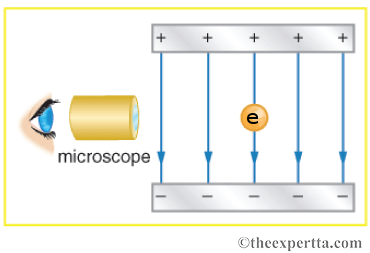
\includegraphics[width=0.5\textwidth]{ex2.png}
\caption{\label{fig:ex2}}
\end{figure}
\small 
If the field were increased in magnitude, the charges would:
\begin{itemize}
\item A: accelerate upwards
\item B: accelerate downwards
\item C: move down at constant v
\item D: move up at constant v
\end{itemize}
\end{column}
\end{columns}
\end{frame}

\begin{frame}{Review}
\begin{columns}[T]
\begin{column}{0.5\textwidth}
\small
Suppose the capacitances $C_1$, $C_2$, and $C_3$ are all 5 $\mu$F.  What is the total capacitance? \\ \vspace{0.5cm}
Suppose $C_1 = C_2 = 5 \mu$F, but $C_3 = 100 \mu$F.  What is the total capacitance? \\ \vspace{0.5cm}
Suppose a 1 $\mu$F capacitor is connected in series with a $1$ k$\Omega$ resistor.  What is the RC time? \\ \vspace{0.5cm}
When will the capacitor in the RC circuit reach 90\% of the votlage of the charging battery?
\end{column}
\begin{column}{0.5\textwidth}
\begin{figure}
\centering
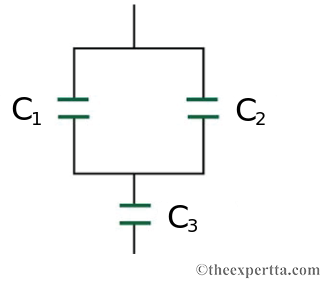
\includegraphics[width=0.95\textwidth]{ex3.png}
\caption{\label{fig:ex3}}
\end{figure}
\end{column}
\end{columns}
\end{frame}

\begin{frame}{Review}
\begin{columns}[T]
\begin{column}{0.5\textwidth}
\small
What equation do you get when you apply the loop rule to the loop abcdefgha, in terms of the variables in the figure? \\ \vspace{0.5cm}
If the current through the top branch is $I_2$ = 0.52 A, what is the current through the bottom, $I_3$, in amps? 
\end{column}
\begin{column}{0.5\textwidth}
\begin{figure}
\centering
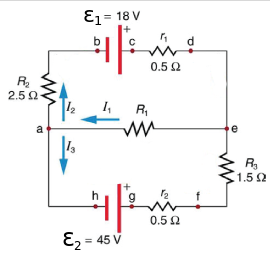
\includegraphics[width=0.95\textwidth]{ex4.png}
\caption{\label{fig:ex4}}
\end{figure}
\end{column}
\end{columns}
\end{frame}

\begin{frame}{Review}
\begin{columns}[T]
\begin{column}{0.65\textwidth}
\small
What is the value of the B-field a distance of 1 cm from a 10A current? \\ \vspace{0.5cm}
If the current is cut in half, but the distance is doubled, what is the new B-field? \\ \vspace{0.5cm}
If two currents flowing in the same direction are placed near each other, they:
\begin{itemize}
\item A: repel each other always
\item B: attract each other always
\item C: repel each other if one changes
\item D: attract each other if one changes
\end{itemize}
\end{column}
\begin{column}{0.35\textwidth}
\begin{figure}
\centering
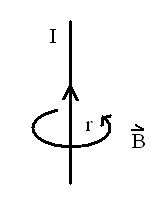
\includegraphics[width=0.95\textwidth]{ex5.png}
\caption{\label{fig:ex5}}
\end{figure}
\end{column}
\end{columns}
\end{frame}

\begin{frame}{Review}
\begin{columns}[T]
\begin{column}{0.65\textwidth}
\small
If the total number of turns in the loop is 500, and the frequency is 1000 Hz, what is the peak emf in the 0.03 T B-field? \\ \vspace{0.5cm}
Double the frequency, $f$, will
\begin{itemize}
\item A: Make the graph at bottom right oscillate more rapidly, but not raise the amplitude.
\item B: Raise the amplitude of the graph at bottom right.
\item C: Lower the amplitude of the graph at bottom right.
\item D: Both raise the amplitude of the graph at bottom right, and make it oscillate more rapidly.
\end{itemize}
\end{column}
\begin{column}{0.35\textwidth}
\begin{figure}
\centering
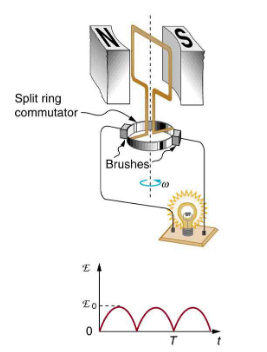
\includegraphics[width=0.95\textwidth]{ex6.png}
\caption{\label{fig:ex6}}
\end{figure}
\end{column}
\end{columns}
\end{frame}

\section{Conclusion}

\begin{frame}{Summary}
\begin{enumerate}
\item Chapter 18 - Charges and Electric Fields
\item Chapter 19 - Electric Potential and Electric Field
\item Chapter 20 - Electric Current, Resistance, and Ohm's Law
\item Chapter 21 - Circuits and DC instruments
\item Chapter 22 - Magnetism
\item Chapter 23 - Electromagnetic Induction
\item Electromagnetic waves
\end{enumerate}
\end{frame}

\end{document}
